% !TeX root = ../rvmonitor.tex

\section{Multi-Head}
\label{sec:multi_head}

\section{Original Approach}

\begin{figure}[!h]
	\centering
	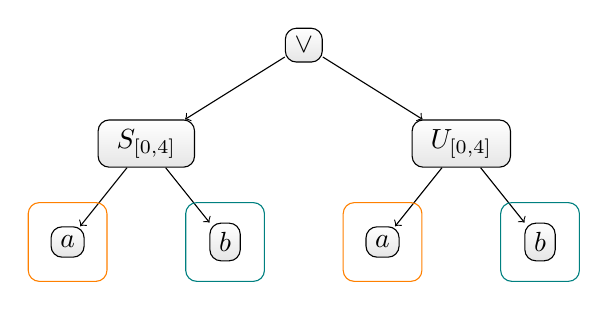
\begin{tikzpicture}[vertex/.style={shape=rectangle, rounded corners,
			draw, align=center,
			top color=white, bottom color=gray!20}]
		\tikzset{edge/.style = {-> = latex'}}
		% Vertices
		\node[vertex] (root1) at (0,0) {$\lor$};
		\node[vertex] (child1) at (-2,-1.25) {$~S_{[0,4]}~$};
		\node[vertex] (child2) at (2,-1.25) {$~U_{[0,4]}~$};
		\node[vertex] (child3) at (-3,-2.5) {$a$};
		\node[vertex] (child4) at (-1,-2.5) {$b$};
		\node[vertex] (child5) at (1,-2.5) {$a$};
		\node[vertex] (child6) at (3,-2.5) {$b$};
		% Edges
		\draw[edge] (root1) to (child1);
		\draw[edge] (root1) to (child2);
		\draw[edge] (child1) to (child3);
		\draw[edge] (child1) to (child4);
		\draw[edge] (child2) to (child5);
		\draw[edge] (child2) to (child6);
		
		\draw[draw=orange, rounded corners] (-3.5,-3) rectangle ++(1,1.0) ;
		\draw[draw=teal, rounded corners] (-1.5,-3) rectangle ++(1,1.0) ;
		\draw[draw=orange, rounded corners] (0.5,-3) rectangle ++(1,1.0) ;
		\draw[draw=teal, rounded corners] (2.5,-3) rectangle ++(1,1.0) ;
	\end{tikzpicture}
\end{figure}





\begin{itemize}
	\item Individual monitor for each node of expression tree: $\strongNext$, $\since$, $\land$, $\lor$, $\neg$, ... 
	\item Efficient caching and representation of temporary information 
	\item Two main steps for each monitor: 
	\begin{enumerate}
		\item Execution of submonitors
		\item Combination of verdicts based on own semantic
	\end{enumerate}
	
\end{itemize}
\begin{figure}[!h]
	\centering
	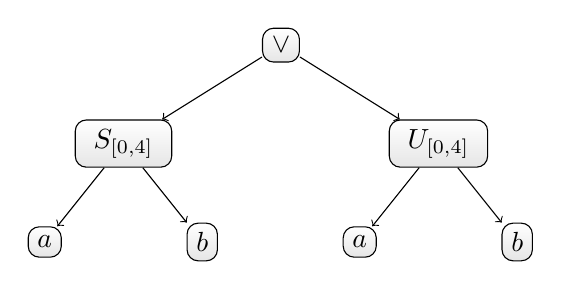
\begin{tikzpicture}[vertex/.style={shape=rectangle, rounded corners,
			draw, align=center,
			top color=white, bottom color=gray!20}]
		\tikzset{edge/.style = {-> = latex'}}
		% Vertices
		\node[vertex] (root1) at (0,0) {$\lor$};
		\node[vertex] (child1) at (-2,-1.25) {$~S_{[0,4]}~$};
		\node[vertex] (child2) at (2,-1.25) {$~U_{[0,4]}~$};
		\node[vertex] (child3) at (-3,-2.5) {$a$};
		\node[vertex] (child4) at (-1,-2.5) {$b$};
		\node[vertex] (child5) at (1,-2.5) {$a$};
		\node[vertex] (child6) at (3,-2.5) {$b$};
		% Edges
		\draw[edge] (root1) to (child1);
		\draw[edge] (root1) to (child2);
		\draw[edge] (child1) to (child3);
		\draw[edge] (child1) to (child4);
		\draw[edge] (child2) to (child5);
		\draw[edge] (child2) to (child6);
		
		
	\end{tikzpicture}
\end{figure}




A multi-head monitor is a tuple $M = (P, V, \kappa, Q, q_0, \delta)$, where $P$ is a non-empty finite set of atomic predicates, $V$ is a verdict alphabet, $\kappa \in \mathbb{N}$ is the number of one-
way (reading) heads, $Q$ is a set of states, $q_0 \in Q$ is an initial state, and $\delta : Q \times E \kappa \implies Q \times
{0, 1} \kappa × (V \cup {\bot})$ is a step function that maps a state and the events read by the heads
to a new state, offsets that indicate which heads to advance, and an optional verdict.




\textbf{Specification}: $(a~S_{[0,4]}~b) \lor (a~U_{[0,4]}~b)$ 
\newline \newline
\textbf{Verdicts:} \\
$a~S_{[0,4]}~b$: (0, ff), (0, ff), (2, ff), (4, tt), (5, tt), (10, tt)  \\
$a~U_{[0,4]}~b$: (0, tt), (0, tt), (2, tt), (4, tt), (5, ff), (10, tt)

\begin{figure*}[!h]
	\centering
	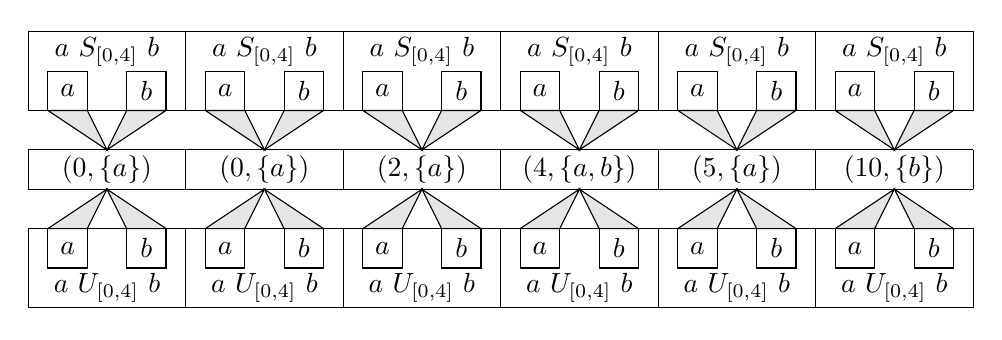
\begin{tikzpicture}
		\draw[xstep=2cm,ystep=0.5cm,black] (0,0) grid (12,0.5);
		\draw (1, 0.25) node{$(0, \{a\})$};
		\draw (3, 0.25) node{$(0, \{a\})$};
		\draw (5, 0.25) node{$(2, \{a\})$};
		\draw (7, 0.25) node{$(4, \{a, b\})$};
		\draw (9, 0.25) node{$(5, \{a\})$};
		\draw (11, 0.25) node{$(10, \{b\})$};
		
		
	
			\draw[draw=black] (0,1) rectangle ++(2,1.0);
			\draw (1, 1.75) node{$a~S_{[0,4]}~b$};
			\draw[draw=black] (0.25,1) rectangle ++(0.5,0.5);
			\draw (0.5, 1.25) node{$a$};
			\draw[draw=black] (1.25,1) rectangle ++(0.5,0.5);
			\draw (1.5, 1.25) node{$b$};
			
			\node (n00) at ( 0.25,  1.0) {}; % root
			\node (n01) at ( 0.75, 1.0) {}; % extreme
			\node (n02) at ( 1.0, 0.5) {}; % extreme
			\fill[fill=gray!20, draw=black] (n00.center)--(n01.center)--(n02.center)--(n00.center);
			\node (n10) at ( 1.25,  1.0) {}; % root
			\node (n11) at ( 1.75, 1.0) {}; % extreme
			\node (n12) at ( 1.0, 0.5) {}; % extreme
			\fill[fill=gray!20, draw=black] (n10.center)--(n11.center)--(n12.center)--(n10.center);
		
		
	
			\draw[draw=black] (2,1) rectangle ++(2,1.0);
			\draw (3, 1.75) node{$a~S_{[0,4]}~b$};
			\draw[draw=black] (2.25,1) rectangle ++(0.5,0.5);
			\draw (2.5, 1.25) node{$a$};
			\draw[draw=black] (3.25,1) rectangle ++(0.5,0.5);
			\draw (3.5, 1.25) node{$b$};
			
			\node (n00) at ( 2.25,  1.0) {}; % root
			\node (n01) at ( 2.75, 1.0) {}; % extreme
			\node (n02) at ( 3.0, 0.5) {}; % extreme
			\fill[fill=gray!20, draw=black] (n00.center)--(n01.center)--(n02.center)--(n00.center);
			\node (n10) at ( 3.25,  1.0) {}; % root
			\node (n11) at ( 3.75, 1.0) {}; % extreme
			\node (n12) at ( 3.0, 0.5) {}; % extreme
			\fill[fill=gray!20, draw=black] (n10.center)--(n11.center)--(n12.center)--(n10.center);
		
		
	
			\draw[draw=black] (4,1) rectangle ++(2,1.0);
			\draw (5, 1.75) node{$a~S_{[0,4]}~b$};
			\draw[draw=black] (4.25,1) rectangle ++(0.5,0.5);
			\draw (4.5, 1.25) node{$a$};
			\draw[draw=black] (5.25,1) rectangle ++(0.5,0.5);
			\draw (5.5, 1.25) node{$b$};
			
			\node (n00) at ( 4.25,  1.0) {}; % root
			\node (n01) at ( 4.75, 1.0) {}; % extreme
			\node (n02) at ( 5.0, 0.5) {}; % extreme
			\fill[fill=gray!20, draw=black] (n00.center)--(n01.center)--(n02.center)--(n00.center);
			\node (n10) at ( 5.25,  1.0) {}; % root
			\node (n11) at ( 5.75, 1.0) {}; % extreme
			\node (n12) at ( 5.0, 0.5) {}; % extreme
			\fill[fill=gray!20, draw=black] (n10.center)--(n11.center)--(n12.center)--(n10.center);
		
		
	
			\draw[draw=black] (6,1) rectangle ++(2,1.0);
			\draw (7, 1.75) node{$a~S_{[0,4]}~b$};
			\draw[draw=black] (6.25,1) rectangle ++(0.5,0.5);
			\draw (6.5, 1.25) node{$a$};
			\draw[draw=black] (7.25,1) rectangle ++(0.5,0.5);
			\draw (7.5, 1.25) node{$b$};
			
			\node (n00) at ( 6.25,  1.0) {}; % root
			\node (n01) at ( 6.75, 1.0) {}; % extreme
			\node (n02) at ( 7.0, 0.5) {}; % extreme
			\fill[fill=gray!20, draw=black] (n00.center)--(n01.center)--(n02.center)--(n00.center);
			\node (n10) at ( 7.25,  1.0) {}; % root
			\node (n11) at ( 7.75, 1.0) {}; % extreme
			\node (n12) at ( 7.0, 0.5) {}; % extreme
			\fill[fill=gray!20, draw=black] (n10.center)--(n11.center)--(n12.center)--(n10.center);
		
		
	
			\draw[draw=black] (8,1) rectangle ++(2,1.0);
			\draw (9, 1.75) node{$a~S_{[0,4]}~b$};
			\draw[draw=black] (8.25,1) rectangle ++(0.5,0.5);
			\draw (8.5, 1.25) node{$a$};
			\draw[draw=black] (9.25,1) rectangle ++(0.5,0.5);
			\draw (9.5, 1.25) node{$b$};
			
			\node (n00) at ( 8.25,  1.0) {}; % root
			\node (n01) at ( 8.75, 1.0) {}; % extreme
			\node (n02) at ( 9.0, 0.5) {}; % extreme
			\fill[fill=gray!20, draw=black] (n00.center)--(n01.center)--(n02.center)--(n00.center);
			\node (n10) at ( 9.25,  1.0) {}; % root
			\node (n11) at ( 9.75, 1.0) {}; % extreme
			\node (n12) at ( 9.0, 0.5) {}; % extreme
			\fill[fill=gray!20, draw=black] (n10.center)--(n11.center)--(n12.center)--(n10.center);
		
		
	
			\draw[draw=black] (10,1) rectangle ++(2,1.0);
			\draw (11, 1.75) node{$a~S_{[0,4]}~b$};
			\draw[draw=black] (10.25,1) rectangle ++(0.5,0.5);
			\draw (10.5, 1.25) node{$a$};
			\draw[draw=black] (11.25,1) rectangle ++(0.5,0.5);
			\draw (11.5, 1.25) node{$b$};
			
			\node (n00) at ( 10.25,  1.0) {}; % root
			\node (n01) at ( 10.75, 1.0) {}; % extreme
			\node (n02) at ( 11.0, 0.5) {}; % extreme
			\fill[fill=gray!20, draw=black] (n00.center)--(n01.center)--(n02.center)--(n00.center);
			\node (n10) at ( 11.25,  1.0) {}; % root
			\node (n11) at ( 11.75, 1.0) {}; % extreme
			\node (n12) at ( 11.0, 0.5) {}; % extreme
			\fill[fill=gray!20, draw=black] (n10.center)--(n11.center)--(n12.center)--(n10.center);
		
		
		
		
		
		
	
			\draw[draw=black] (0,-1.5) rectangle ++(2,1.0);
			\draw (1, -1.25) node{$a~U_{[0,4]}~b$};
			\draw[draw=black] (0.25,-1) rectangle ++(0.5,0.5);
			\draw (0.5, -0.75) node{$a$};
			\draw[draw=black] (1.25, -1) rectangle ++(0.5,0.5);
			\draw (1.5, -0.75) node{$b$};
			
			\node (n20) at ( 0.25, -0.5) {}; % root
			\node (n21) at ( 0.75, -0.5) {}; % extreme
			\node (n22) at ( 1.0, -0) {}; % extreme
			\fill[fill=gray!20, draw=black] (n20.center)--(n21.center)--(n22.center)--(n20.center);
			
			\node (n30) at ( 1.25,  -0.5) {}; % root
			\node (n31) at ( 1.75, -0.5) {}; % extreme
			\node (n32) at ( 1.0, 0) {}; % extreme
			\fill[fill=gray!20, draw=black] (n30.center)--(n31.center)--(n32.center)--(n30.center);
		
		
	
			\draw[draw=black] (2,-1.5) rectangle ++(2,1.0);
			\draw (3, -1.25) node{$a~U_{[0,4]}~b$};
			\draw[draw=black] (2.25,-1) rectangle ++(0.5,0.5);
			\draw (2.5, -0.75) node{$a$};
			\draw[draw=black] (3.25, -1) rectangle ++(0.5,0.5);
			\draw (3.5, -0.75) node{$b$};
			
			\node (n20) at ( 2.25, -0.5) {}; % root
			\node (n21) at ( 2.75, -0.5) {}; % extreme
			\node (n22) at ( 3.0, -0) {}; % extreme
			\fill[fill=gray!20, draw=black] (n20.center)--(n21.center)--(n22.center)--(n20.center);
			
			\node (n30) at ( 3.25,  -0.5) {}; % root
			\node (n31) at ( 3.75, -0.5) {}; % extreme
			\node (n32) at ( 3.0, 0) {}; % extreme
			\fill[fill=gray!20, draw=black] (n30.center)--(n31.center)--(n32.center)--(n30.center);
		
		
	
			\draw[draw=black] (4,-1.5) rectangle ++(2,1.0);
			\draw (5, -1.25) node{$a~U_{[0,4]}~b$};
			\draw[draw=black] (4.25,-1) rectangle ++(0.5,0.5);
			\draw (4.5, -0.75) node{$a$};
			\draw[draw=black] (5.25, -1) rectangle ++(0.5,0.5);
			\draw (5.5, -0.75) node{$b$};
			
			\node (n20) at ( 4.25, -0.5) {}; % root
			\node (n21) at ( 4.75, -0.5) {}; % extreme
			\node (n22) at ( 5.0, -0) {}; % extreme
			\fill[fill=gray!20, draw=black] (n20.center)--(n21.center)--(n22.center)--(n20.center);
			
			\node (n30) at ( 5.25,  -0.5) {}; % root
			\node (n31) at ( 5.75, -0.5) {}; % extreme
			\node (n32) at ( 5.0, 0) {}; % extreme
			\fill[fill=gray!20, draw=black] (n30.center)--(n31.center)--(n32.center)--(n30.center);
		
		
	
			\draw[draw=black] (6,-1.5) rectangle ++(2,1.0);
			\draw (7, -1.25) node{$a~U_{[0,4]}~b$};
			\draw[draw=black] (6.25,-1) rectangle ++(0.5,0.5);
			\draw (6.5, -0.75) node{$a$};
			\draw[draw=black] (7.25, -1) rectangle ++(0.5,0.5);
			\draw (7.5, -0.75) node{$b$};
			
			\node (n20) at ( 6.25, -0.5) {}; % root
			\node (n21) at ( 6.75, -0.5) {}; % extreme
			\node (n22) at ( 7.0, -0) {}; % extreme
			\fill[fill=gray!20, draw=black] (n20.center)--(n21.center)--(n22.center)--(n20.center);
			
			\node (n30) at ( 7.25,  -0.5) {}; % root
			\node (n31) at ( 7.75, -0.5) {}; % extreme
			\node (n32) at ( 7.0, 0) {}; % extreme
			\fill[fill=gray!20, draw=black] (n30.center)--(n31.center)--(n32.center)--(n30.center);
		
		
	
			\draw[draw=black] (8,-1.5) rectangle ++(2,1.0);
			\draw (9, -1.25) node{$a~U_{[0,4]}~b$};
			\draw[draw=black] (8.25,-1) rectangle ++(0.5,0.5);
			\draw (8.5, -0.75) node{$a$};
			\draw[draw=black] (9.25, -1) rectangle ++(0.5,0.5);
			\draw (9.5, -0.75) node{$b$};
			
			\node (n20) at ( 8.25, -0.5) {}; % root
			\node (n21) at ( 8.75, -0.5) {}; % extreme
			\node (n22) at ( 9.0, -0) {}; % extreme
			\fill[fill=gray!20, draw=black] (n20.center)--(n21.center)--(n22.center)--(n20.center);
			
			\node (n30) at ( 9.25,  -0.5) {}; % root
			\node (n31) at ( 9.75, -0.5) {}; % extreme
			\node (n32) at ( 9.0, 0) {}; % extreme
			\fill[fill=gray!20, draw=black] (n30.center)--(n31.center)--(n32.center)--(n30.center);
		
		
	
			\draw[draw=black] (10,-1.5) rectangle ++(2,1.0);
			\draw (11, -1.25) node{$a~U_{[0,4]}~b$};
			\draw[draw=black] (10.25,-1) rectangle ++(0.5,0.5);
			\draw (10.5, -0.75) node{$a$};
			\draw[draw=black] (11.25, -1) rectangle ++(0.5,0.5);
			\draw (11.5, -0.75) node{$b$};
			
			\node (n20) at ( 10.25, -0.5) {}; % root
			\node (n21) at ( 10.75, -0.5) {}; % extreme
			\node (n22) at ( 11.0, -0) {}; % extreme
			\fill[fill=gray!20, draw=black] (n20.center)--(n21.center)--(n22.center)--(n20.center);
			
			\node (n30) at ( 11.25,  -0.5) {}; % root
			\node (n31) at ( 11.75, -0.5) {}; % extreme
			\node (n32) at ( 11.0, 0) {}; % extreme
			\fill[fill=gray!20, draw=black] (n30.center)--(n31.center)--(n32.center)--(n30.center);
		
		
		
	\end{tikzpicture}
\end{figure*}   





Advantages:
\begin{itemize}
	\setlength\itemsep{0.75cm}
	\item Verdict for each time-stamp
	\item Arbitrary combination of past and future operators
	\item Very efficient for single specifications
\end{itemize}
\vspace{0.5cm}
Disadvantage:
\begin{itemize}
	\item Does not reuse information: between and within specifications
\end{itemize}
\vspace{0.5cm}
\hspace{1cm}$\rightarrow$ \textbf{Connected Multi-Head Multi-Root Monitoring}





\textbf{Spec. 1}: $(a~S_{[0,4]}~b) \lor (a~U_{[0,4]}~b)$ 	\newline
\textbf{Spec. 2}: $a~S_{[0,4]}~b $ \newline
\textbf{Spec. 3}: $a~U_{[0,4]}~b$ \newline


	\textit{Multi-Head monitoring} requires three individual monitors:
	\begin{figure}[!h]
		\centering
		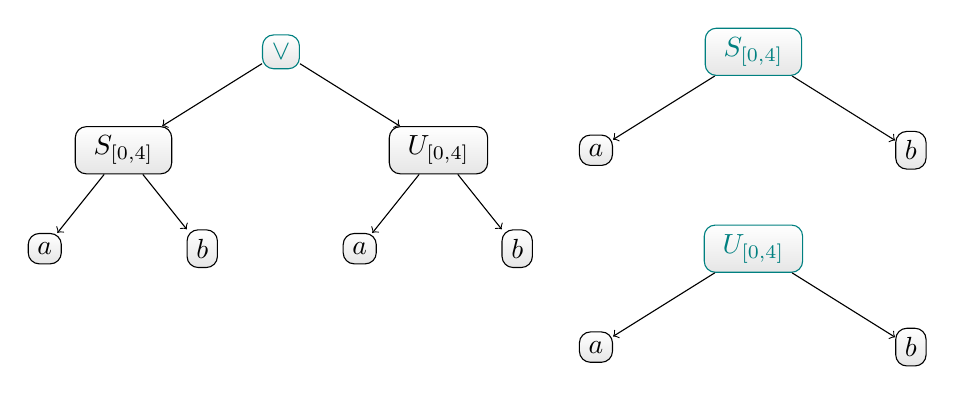
\begin{tikzpicture}[vertex/.style={shape=rectangle, rounded corners,
				draw, align=center,
				top color=white, bottom color=gray!20}]
			\tikzset{edge/.style = {-> = latex'}}
			% Vertices
			\node[vertex, color=teal] (root1) at (0,0) {$\lor$};
			\node[vertex] (child1) at (-2,-1.25) {$~S_{[0,4]}~$};
			\node[vertex] (child2) at (2,-1.25) {$~U_{[0,4]}~$};
			\node[vertex] (child3) at (-3,-2.5) {$a$};
			\node[vertex] (child4) at (-1,-2.5) {$b$};
			\node[vertex] (child5) at (1,-2.5) {$a$};
			\node[vertex] (child6) at (3,-2.5) {$b$};
			% Edges
			\draw[edge] (root1) to (child1);
			\draw[edge] (root1) to (child2);
			\draw[edge] (child1) to (child3);
			\draw[edge] (child1) to (child4);
			\draw[edge] (child2) to (child5);
			\draw[edge] (child2) to (child6);
			
			\node[vertex, color=teal] (root2) at (6,0) {$~S_{[0,4]}~$};
			\node[vertex] (child5) at (4,-1.25) {$a$};
			\node[vertex] (child6) at (8,-1.25) {$b$};
			\draw[edge] (root2) to (child5);
			\draw[edge] (root2) to (child6);
			
			\node[vertex, color=teal] (root3) at (6,-2.5) {$~U_{[0,4]}~$};
			\node[vertex] (child7) at (4,-3.75) {$a$};
			\node[vertex] (child8) at (8,-3.75) {$b$};
			\draw[edge] (root3) to (child7);
			\draw[edge] (root3) to (child8);
		\end{tikzpicture}
\end{figure}

	\textit{Connected Multi-Head Multi-Root monitoring} requires only one monitor:
	\begin{figure}[!h]
		\centering
		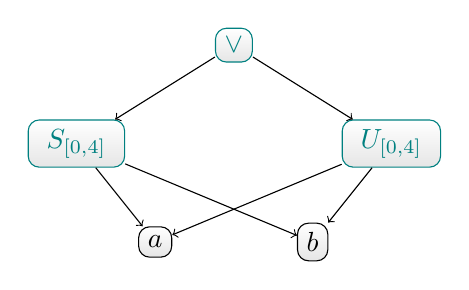
\begin{tikzpicture}[vertex/.style={shape=rectangle, rounded corners,
				draw, align=center,
				top color=white, bottom color=gray!20}]
			\tikzset{edge/.style = {-> = latex'}}
			% Vertices
			\node[vertex, color=teal] (root1) at (0,0) {$\lor$};
			\node[vertex, color=teal] (child1) at (-2,-1.25) {$~S_{[0,4]}~$};
			\node[vertex, color=teal] (child2) at (2,-1.25) {$~U_{[0,4]}~$};
			\node[vertex] (child3) at (-1,-2.5) {$a$};
			\node[vertex] (child4) at (1,-2.5) {$b$};
			% Edges
			\draw[edge] (root1) to (child1);
			\draw[edge] (root1) to (child2);
			\draw[edge] (child1) to (child3);
			\draw[edge] (child1) to (child4);
			\draw[edge] (child2) to (child3);
			\draw[edge] (child2) to (child4);
			
			
		\end{tikzpicture}
	\end{figure}

